%%%%%%%%%%%%%%%%%%%%%%%%%%%%%%%%%%%%%%%%%%%%%%%%%%%%%%%%%%%%%%%
%
% Welcome to writeLaTeX --- just edit your LaTeX on the left,
% and we'll compile it for you on the right. If you give 
% someone the link to this page, they can edit at the same
% time. See the help menu above for more info. Enjoy!
%
%%%%%%%%%%%%%%%%%%%%%%%%%%%%%%%%%%%%%%%%%%%%%%%%%%%%%%%%%%%%%%%

% --------------------------------------------------------------
% This is all preamble stuff that you don't have to worry about.
% Head down to where it says "Start here"
% --------------------------------------------------------------
 
\documentclass[12pt]{article}

\usepackage{graphicx}
\graphicspath{{Images/}{./}} % Specifies where to look for included images (trailing slash required)

\usepackage[spanish]{babel}
\usepackage[margin=1in]{geometry} 
\usepackage{amsmath,amsthm,amssymb}
\usepackage[ruled,vlined]{algorithm2e}
\usepackage{xcolor}
\usepackage{array} % needed for \arraybackslash

\usepackage{adjustbox} % for \adjincludegraphics

\usepackage{subcaption}
\usepackage{bibentry}
%\bibliographystyle{apalike}
\usepackage{chngcntr}
\usepackage{lipsum}% http://ctan.org/pkg/lipsum
\usepackage{hanging}% http://ctan.org/pkg/hanging

\usepackage{xcolor,colortbl}
\usepackage{multirow}

\usepackage{animate}
\usepackage{multicol}
\usepackage{tabularx,booktabs}
\usepackage{forloop}
\usepackage{ragged2e}

\usepackage{bbding} %palomitas checkmark
\usepackage{pifont}
\usepackage{lipsum,tabularx}

\newcommand{\N}{\mathbb{N}}
\newcommand{\Z}{\mathbb{Z}}
 
\newenvironment{theorem}[2][Theorem]{\begin{trivlist}
\item[\hskip \labelsep {\bfseries #1}\hskip \labelsep {\bfseries #2.}]}{\end{trivlist}}
\newenvironment{lemma}[2][Lemma]{\begin{trivlist}
\item[\hskip \labelsep {\bfseries #1}\hskip \labelsep {\bfseries #2.}]}{\end{trivlist}}
\newenvironment{exercise}[2][Exercise]{\begin{trivlist}
\item[\hskip \labelsep {\bfseries #1}\hskip \labelsep {\bfseries #2.}]}{\end{trivlist}}
\newenvironment{problem}[2][Problem]{\begin{trivlist}
\item[\hskip \labelsep {\bfseries #1}\hskip \labelsep {\bfseries #2.}]}{\end{trivlist}}
\newenvironment{question}[2][Question]{\begin{trivlist}
\item[\hskip \labelsep {\bfseries #1}\hskip \labelsep {\bfseries #2.}]}{\end{trivlist}}
\newenvironment{corollary}[2][Corollary]{\begin{trivlist}
\item[\hskip \labelsep {\bfseries #1}\hskip \labelsep {\bfseries #2.}]}{\end{trivlist}}

\newenvironment{solution}{\begin{proof}[Solution]}{\end{proof}}
 
\begin{document}
 
% --------------------------------------------------------------
%                         Start here
% --------------------------------------------------------------
 
\title{Estrategias para la exploración coordinada multi-VANT}%replace X with the appropriate number
\author{Luis Ballado} %if necessary, replace with your course title
 
\maketitle

\begin{itemize}
\item Al explorar se descubrirán nuevas fronteras, que serán las que se ofertarán al conjunto de robots en base a su posición en un instante de tiempo $t$, sin perder el rango de comunicación. 
\item No es una asignación balanceada. La lista de fronteras crecerá, y los robots no.\\
  En la tesis para robots terrestres (Juan-Carlos), se balancea creando robots virtuales al momento de auto-ofertar y seleccionar la siguiente acción a efectuar el robot.
\end{itemize}

\vspace{1cm}
\hrule
\vspace{1cm}

La exploración autónoma es una tarea fundamental en el campo de la robótica. Para lograrlo, es necesario resolver los siguientes sistemas.

%INCLUIR IMAGEN EXPLORACIO
\begin{center}
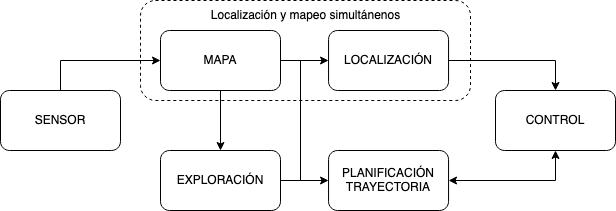
\includegraphics[width=0.7\textwidth]{exploracion}
\end{center}
\vspace{0.5cm}
Dado un conjunto de Vehículos Aéreos No Tripulados (VANT) denotados como $V = {V_{1}, V_{2}, V_{3},...,V_{n}}$, cuya posición inicial es conocida y se desplazan a través de un medio ambiente tridimensional desconocido. Se considera que los VANTS resuelven los problemas de navegación autónoma, es decir cuentan con sistema de percepción, sistema de localización y mapeo simultáneos, sistema de planificación de trayectorias y sistema de control para su navegación. \\

\newpage

Un VANT cuenta con seis grados de libertad (x, y, z, roll, pitch, yaw) \\

El estado de un VANT (considerando las velocidades), se puede denotar como:\\
\[
R = \{x, y, z, \phi, \theta, \psi, \dot{x}, \dot{y}, \dot{z}, \dot{\phi}, \dot{\theta}, \dot{\psi}\}^T
\]

Se descubrirán nuevas fronteras que se ofertarán a un número limitado de VANT.\\

La localización del robot $x_{t}^{r}$, se denota por el índice $r$ en un instante de tiempo $t$.

\[
X_{T}^{r} = {x_{0}^{r},x_{1}^{r},x_{2}^{r},...,x_{T}^{r}}
\]

\begin{itemize}
\item $x_{t}^{r}$ - donde $t$ es un tiempo finito y la ubicación inicial de cada robot es conocida.
\item $u_{t}^{r}$ - la odometría provee información entre dos posiciones consecutivas.
\item $z_{t}^{r}$ - cada robot percibe el medio ambiente.
\end{itemize}

Cada VANT puede comunicarse directamente con cualquier otro dentro de un rango de comunicación $\beta$ con centro del robot.\\

\begin{center}
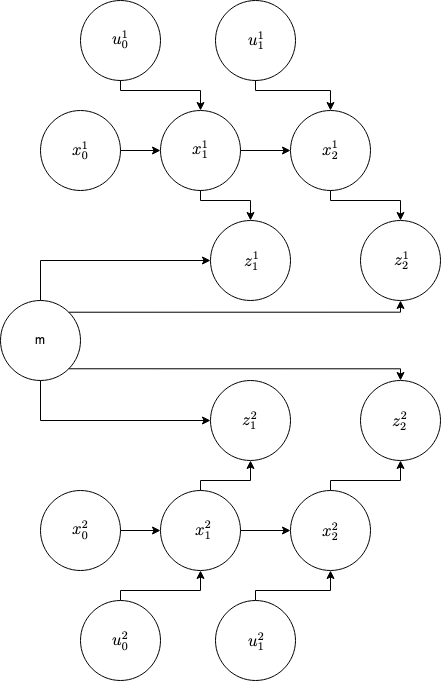
\includegraphics[width=0.55\textwidth]{diagrama}
\end{center}

El problema se puede formular dado un conjunto de robots y un conjunto de fronteras a explorar, el objetivo consiste en asegurar asignaciones eficientes que minimicen el tiempo total de exploración.\\

Se considera tomar un enfoque de auto-ofertas de mercado guiandose de la información de la posición de los demás robot y la actualización del mapa proporcionada por cada robot.\\

Las tareas (fronteras) son independientes 

\end{document}
